\documentclass[11pt]{easymemo3}

\SectionNumber
%\BlackAndWhite

\begin{document}

\MakeTitle{2025.3.11}{クラスター多極子基底}{明大理工 楠瀬博明}


\section{クラスター}

サイトやボンドのクラスター多極子基底を構築するために、球面を離散化してその離散点で球面調和関数を評価することで多極子基底を構築する。
さらに結晶点群や空間群におけるWyckoff位置からなるクラスター上での多極子基底を、対称操作に基づくマッピングにより生成する。

\subsection{ルートクラスター}

多極子基底は半径1の球面上で定義されるので、球面を離散化して関数を評価する。
連続回転群から低下した点群を念頭においているため、用いたい点群のうち最大の対称性をもつ点群の一般点が含まれるように離散点を選ぶ。
ここでは、32の結晶点群を考えるため、$O_{\rm h}$と$D_{\rm 6h}$の一般点を考えれば十分である。

\begin{figure}[!htb]
\begin{center}
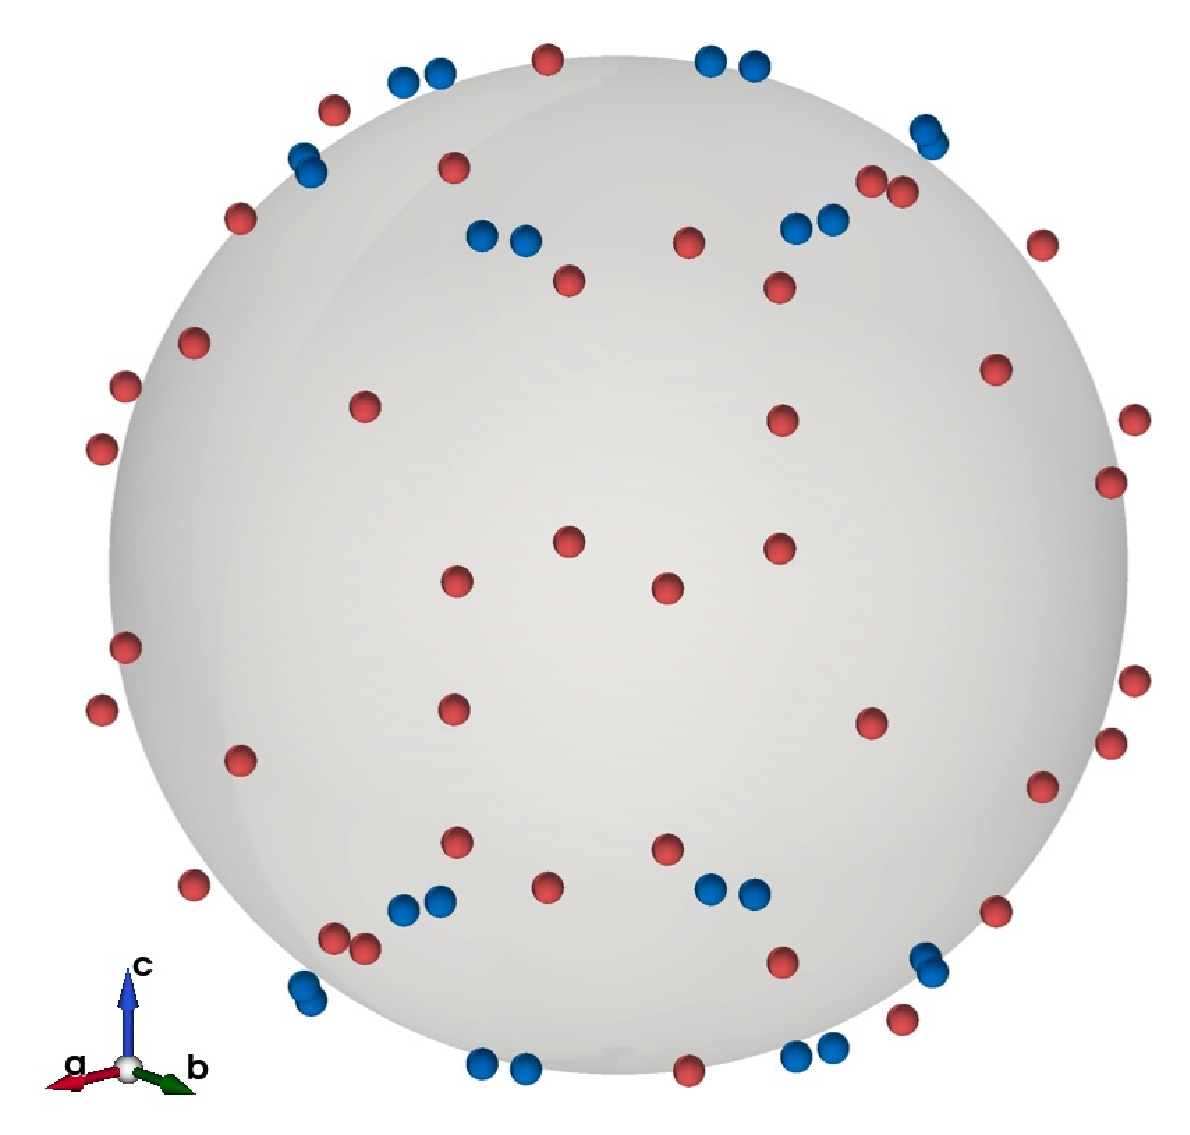
\includegraphics[width=7cm]{fig/rc_site.eps}
\end{center}
\caption{ルートクラスター ($O_{\rm h}$:赤, $D_{\rm 6h}$:青)。}
\label{fig_rc_site}
\end{figure}

代表点(生成される点が一般点になるように選ぶ)を$\bm{r}_0$とし、各点群の対称操作$\mathcal{G}_j$ ($j=1,2,\cdots,N$)を$\bm{r}_0$に作用して得られる点の集合を$\set{\bm{r}_j}$とする(図\ref{fig_rc_site})。
対称操作によって得られる点は重複する場合があるので、それらは取り除き、$i\to j$の対応表も求めておく。
この離散点からなるクラスターをルートクラスターと呼ぶ。
$O_{\rm h}$と$D_{\rm 6h}$の点群の場合、クラスターのサイト数は$N=64$、重複8点である(その対称操作は、$1$, $\bar{1}$, $2_{100}$, $2_{010}=2_{120}$, $m_{100}$, $m_{010}=m_{120}$, $2_{001}$, $m_{001}$)。
\texttt{MultiPie}では、$\bm{r}_{0}=\frac{1}{4\sqrt{2}}(5,\sqrt{3},2)$ [$\bm{r}_{0}=1$]を採用した。
空間群のWyckoff位置のデフォルト値として使用するときは、分率座標の範囲に制限が加わる場合があるので、どの場合でも範囲に収まるよう$\bm{r}_{0}/5$を用いる。

なお、孤立分子を取り扱う場合は、結晶点群ではなく、$O_{\rm h}$, $I_{\rm h}$および$D_{\rm nh}$, $D_{\rm nd}$ ($n=7,8,9,10,11,12$)の一般点を用いる。この選択により、これらの部分群である32の結晶点群と$C_{\rm n}$, $C_{\rm nv}$, $C_{\rm nh}$, $D_{\rm n}$, $D_{\rm nh}$, $D_{\rm nd}$, $S_{\rm 2n}$ ($n=12$以下), $I$, $I_{\rm h}$の点群を扱うことができる。
同様に、より高次の点群についても拡張できる。

\subsection{Wyckoffクラスター}

各結晶点群と空間群に対する多極子基底のクラスター表現は、対称操作で関係づけられるサイトまたはボンドのクラスター空間で定義される。
対称操作とクラスターの各成分のマッピングを用いて、ルートクラスターの表現からWyckoffクラスターへマッピングを行うことにより、多極子基底のWyckoffクラスター表現が得られる。
なお、対称操作の並進を除く部分は、空間群と対応点群で共通の順序を用いる。

\subsubsection{サイト・クラスター}

サイトのWyckoffクラスターは、ITAに掲載されているWyckoff位置を用いればよい。
サイト・クラスターの構成点$\bm{s}_{i}$ (分率座標)と対称操作$j$のマッピング$m_{i}=\{j\}$を生成しておく。

\subsubsection{ボンド・クラスター}
ボンドのWyckoffクラスターは、ボンド中心についてはサイトのWyckoff位置と共通である。
ボンドは向きがあるので、同じ位置に複数個の組み合わせが現れる場合があり、ボンド・クラスターの成分数はサイト・クラスターの成分数と等しいかそれより大きい。
そのため、ボンドクラスターを(ボンドWyckoff)@(サイトWyckoff)のように表現する。
ボンド・クラスターの構成構成ボンド$\bm{v}_{i}@\bm{c}_{i}$ (どちらも分率座標)とマッピング$m_{i}=\{j\}$を生成しておく。
ただし、マッピングにおいてボンドの向きが逆になる場合は$-j$とする。

全ての結晶点群と空間群についてボンド・クラスターを生成する方法については最後に述べる。


\section{多極子基底のクラスター表現}

\subsection{ルートクラスター表現}

ルートクラスターの構成点$\{\bm{r}_{j}\}$に対して、結晶点群の多極子調和関数$\vec{Q}_{l,\gamma}^{(\Gamma,n;s,k)}(\bm{r};\vec{q})$, $\vec{G}_{l,\gamma}^{(\Gamma,n;s,k)}(\bm{r};\vec{q})$を$s=0,1$について評価する。
これらを
\begin{align}
&
\mathbb{Q}_{l,\gamma}^{(\Gamma,n)}=\biggl[\vec{Q}_{l,\gamma}^{(\Gamma,n;0,0)}(\bm{r}_{1};\vec{q}),\vec{Q}_{l,\gamma}^{(\Gamma,n;0,0)}(\bm{r}_{2};\vec{q}),\cdots,\vec{Q}_{l,\gamma}^{(\Gamma,n;0,0)}(\bm{r}_{N};\vec{q})\biggr],
\\&
\vec{\mathbb{Q}}_{l,\gamma}^{(\Gamma,n,\mp1)}=\biggl[\vec{Q}_{l,\gamma}^{(\Gamma,n;1,\mp1)}(\bm{r}_{1};\vec{q}),\vec{Q}_{l,\gamma}^{(\Gamma,n;1,\mp1)}(\bm{r}_{2};\vec{q}),\cdots,\vec{Q}_{l,\gamma}^{(\Gamma,n;1,\mp1)}(\bm{r}_{N};\vec{q})\biggr],
\cr&
\vec{\mathbb{G}}_{l,\gamma}^{(\Gamma,n,0)}=\biggl[\vec{G}_{l,\gamma}^{(\Gamma,n;1,0)}(\bm{r}_{1};\vec{q}),\vec{G}_{l,\gamma}^{(\Gamma,n;1,0)}(\bm{r}_{2};\vec{q}),\cdots,\vec{G}_{l,\gamma}^{(\Gamma,n;1,0)}(\bm{r}_{N};\vec{q})\biggr]
\end{align}
と表す。
$\mathbb{X}_{l,\gamma}^{(\Gamma,n)}$はモノポール調和関数($N$成分ベクトル)、$\vec{\mathbb{X}}_{l,\gamma}^{(\Gamma,n)}(k)$はダイポール調和関数($(N,3)$成分ベクトル)である。


\subsection{Wyckoffクラスター表現}

指定されたWyckoffクラスターに関する多極子基底表現は、マッピングに従ってルートクラスター表現を重ね合わせて得られる。

\subsubsection{サイトクラスター}

サイトクラスターに置く自由度が極性電荷であることを考慮して、$\mathbb{Q}_{l,\gamma}^{(\Gamma,n)}$のルートクラスター表現を用いる。
サイトクラスター位置を$\bm{s}_{i}$ ($i=1,2,\cdots,c$)、マッピングを$m_{i}=\{j\}$とすると
\begin{align}
\overline{\mathbb{Q}}_{l,\gamma}^{{\rm (s)}(\Gamma,n)}=\biggl[
\sum_{j}^{\in m_{1}}\mathbb{Q}_{l,\gamma}^{(\Gamma,n)}(j),
\sum_{j}^{\in m_{2}}\mathbb{Q}_{l,\gamma}^{(\Gamma,n)}(j),
\cdots
\sum_{j}^{\in m_{c}}\mathbb{Q}_{l,\gamma}^{(\Gamma,n)}(j)
\biggr]
\end{align}
により、サイトクラスターに射影した多極子基底表現を生成し、これにGram-Schmidtの正規直交化を行って、Wyckoffクラスターの多極子基底表現$\mathbb{Q}_{l,\gamma}^{{\rm (s)}(\Gamma,n)}$を得る。
正規直交化の際、直交化前の基底を$(\Gamma,l,n,\gamma)$の順に並べておくとよい\footnote{既約表現ごとに直交化されることを考慮し、低ランクの基底を優先するため。}。

\subsubsection{対称ボンドクラスター}

対称ボンドクラスターに置く自由度は極性電荷またはボンド方向を主軸とする極性四極子$Q_{u}$であることを考慮して、$\mathbb{Q}_{l,\gamma}^{(\Gamma,n)}$のルートクラスター表現を用いる。
ボンドクラスターを$\bm{v}_{i}@\bm{c}_{i}$ ($i=1,2,\cdots,c$)、マッピングを$m_{i}=\{j\}$とすると
\begin{align}
\overline{\mathbb{Q}}_{l,\gamma}^{{\rm (sb)}(\Gamma,n)}=\biggl[
\sum_{j}^{\in m_{1}}\mathbb{Q}_{l,\gamma}^{(\Gamma,n)}(|j|),
\sum_{j}^{\in m_{2}}\mathbb{Q}_{l,\gamma}^{(\Gamma,n)}(|j|),
\cdots
\sum_{j}^{\in m_{c}}\mathbb{Q}_{l,\gamma}^{(\Gamma,n)}(|j|)
\biggr]
\end{align}
により、対称ボンドクラスターに射影した多極子基底表現を生成し、これにGram-Schmidtの正規直交化を行って、Wyckoffクラスターの多極子基底表現$\mathbb{Q}_{l,\gamma}^{{\rm (sb)}(\Gamma,n)}$を得る。
正規直交化の際、直交化前の基底を$(\Gamma,l,n,\gamma)$の順に並べておくとよい\footnote{既約表現ごとに直交化されることを考慮し、低ランクの基底を優先するため。}。

\subsubsection{ベクトル・ボンドクラスター}

ボンドクラスターにボンド方向を主軸とする極性双極子$Q_{z}$をそのまま置く場合は、$\vec{\mathbb{Q}}_{l,\gamma}^{(\Gamma,n)}(k)$と$\vec{\mathbb{G}}_{l,\gamma}^{(\Gamma,n)}(k)$のルートクラスター表現を用いる。
ボンドクラスターを$\bm{v}_{i}@\bm{c}_{i}$ ($i=1,2,\cdots,c$)、マッピングを$m_{i}=\{j\}$とすると、ボンドの向きはダイポール調和関数で考慮されているので、そのまま和を取って
\begin{align}
\overline{\vec{\mathbb{X}}}_{l,\gamma}^{{\rm (v)}(\Gamma,n,k)}=\biggl[
\sum_{j}^{\in m_{1}}\vec{\mathbb{X}}_{l,\gamma}^{(\Gamma,n,k)}(|j|),
\sum_{j}^{\in m_{2}}\vec{\mathbb{X}}_{l,\gamma}^{(\Gamma,n,k)}(|j|),
\cdots
\sum_{j}^{\in m_{c}}\vec{\mathbb{X}}_{l,\gamma}^{(\Gamma,n,k)}(|j|)
\biggr]
\end{align}
により、ボンドクラスターに射影したベクトル多極子基底表現を生成し、これにGram-Schmidtの正規直交化を行って、Wyckoffクラスターのベクトル多極子基底表現$\vec{\mathbb{Q}}_{l,\gamma}^{{\rm (v)}(\Gamma,n,\mp1)}$, $\vec{\mathbb{G}}_{l,\gamma}^{{\rm (v)}(\Gamma,n,0)}$を得る。
正規直交化の際、直交化前の基底を$(\Gamma,l,k,n,\gamma)$の順に並べておくとよい\footnote{既約表現ごとに直交化されることを考慮し、低ランクの基底および同ランク内で$k=-1,0,1$基底の順で優先するため。}。

\subsubsection{反対称ボンドクラスター}

反対称ボンドクラスターに置く自由度はボンド方向を主軸とする極性双極子$Q_{z}$であることを考慮して、$\mathbb{Q}_{l,\gamma}^{(\Gamma,n)}$のルートクラスター表現を用いて以下のように生成する\footnote{これはVer.1と同じ生成方法である。}。
${\rm sgn}(j)$の因子はボンドの向きを考慮するためである。
ボンドクラスターを$\bm{v}_{i}@\bm{c}_{i}$ ($i=1,2,\cdots,c$)、マッピングを$m_{i}=\{j\}$とすると
\begin{align}
\overline{\mathbb{Q}}_{l,\gamma}^{{\rm (ab)}(\Gamma,n)}=\biggl[
\sum_{j}^{\in m_{1}}{\rm sgn}(j)\mathbb{Q}_{l,\gamma}^{(\Gamma,n)}(|j|),
\sum_{j}^{\in m_{2}}{\rm sgn}(j)\mathbb{Q}_{l,\gamma}^{(\Gamma,n)}(|j|),
\cdots
\sum_{j}^{\in m_{c}}{\rm sgn}(j)\mathbb{Q}_{l,\gamma}^{(\Gamma,n)}(|j|)
\biggr]
\end{align}
により、反対称ボンドクラスターに射影した多極子基底表現を生成し、これにGram-Schmidtの正規直交化を行って、Wyckoffクラスターの多極子基底表現$\mathbb{Q}_{l,\gamma}^{{\rm (ab)}(\Gamma,n)}$を得る。

このようにして生成した多極子基底のタグは、場合によっては極性$\mathbb{Q}$より軸性$\mathbb{G}$の方が適切である場合がある。
そこで、以下のようにしてタグの付替えを行う。
ボンドの定義$\{\bm{v}_i\}$と基底$\mathbb{Q}_{l,\gamma}^{{\rm (ab)}(\Gamma,n)}$に対して、多極子基底を
\begin{align}
\vec{\mathbb{Q}}_{l,\gamma}^{{\rm (ab)}(\Gamma,n)}=\biggl[
\mathbb{Q}_{l,\gamma}^{{\rm (ab)}(\Gamma,n)}(1)\bm{v}_1,
\mathbb{Q}_{l,\gamma}^{{\rm (ab)}(\Gamma,n)}(2)\bm{v}_2,
\cdots,
\mathbb{Q}_{l,\gamma}^{{\rm (ab)}(\Gamma,n)}(c)\bm{v}_c
\biggr]
\end{align}
のように導入する。
この多極子基底とベクトル・ボンドクラスター表現$\vec{\mathbb{X}}_\alpha=\vec{\mathbb{Q}}_{l,\gamma}^{{\rm (v)}(\Gamma,n,\mp1)}$, $\vec{\mathbb{G}}_{l,\gamma}^{{\rm (v)}(\Gamma,n,0)}$との内積
\begin{align}
c_\alpha =\vec{\mathbb{Q}}_{l,\gamma}^{{\rm (ab)}(\Gamma,n)}\cdot\vec{\mathbb{X}}_\alpha
\end{align}
を求め、$c_\alpha$が有限の重なりを持つ最初のベクトル・ボンドクラスター基底$\alpha$を用いて$\mathbb{Q}_{l,\gamma}^{{\rm (ab)}(\Gamma,n)}\to \mathbb{X}_\alpha$に付け替える。
ただし、既に使用した$\alpha$は除く。

このようにして、Wyckoffクラスターの多極子基底表現$\mathbb{Q}_{l,\gamma}^{{\rm (ab)}(\Gamma,n,\mp1)}$, $\mathbb{G}_{l,\gamma}^{{\rm (ab)}(\Gamma,n,0)}$を得る。
得られた基底は、ベクトル・ボンドクラスター基底$\vec{\mathbb{X}}_\alpha=\vec{\mathbb{Q}}_{l,\gamma}^{{\rm (v)}(\Gamma,n,\mp1)}$, $\vec{\mathbb{G}}_{l,\gamma}^{{\rm (v)}(\Gamma,n,0)}$と同じ順序で並んでいる。




\section{Bond Wyckoffの生成法}

各点群や空間群のサイトのWyckoff位置ごとにbondのWyckoffを生成する。
ただし、点群の{\tt 1o}サイト$(0,0,0)$は除く。
\begin{enumerate}[(1)]
\item
まず、Wyckoff位置の最初のサイトに対して、独立なベクトル方向を生成する。
独立なベクトルになり得る方向として、各結晶系で最も対称性が高い群のWyckoff位置を用いる。
そのとき、向きが反対のものや$(X,Y,Z)$の入れ替えで等価になるものは除く。
また、より変数$(X,Y,Z)$の数が多い一般的な方向を表すベクトルを優先し、その変数に$Y=X$や$X=0$などの制限を課して得られうベクトルを次の優先順位として用意する。

このようにして用意した独立ベクトル候補に対し、Wyckoff位置の最初のサイトにマップされる対称操作を施して、ベクトルのセットを生成する。
向きや順序を一意的に並べ替えて、ベクトルセットの中から重複するものを除く。
また、ベクトルクセットのサイズが同じグループで、変数に$Y=X$や$X=0$の制限を加えて得られるベクトルは除く。
このような手順で、最初のWyckoffサイトに対する独立なベクトルのセットを用意する。

\item 手順(1)で得られたベクトルセットの各々に、2番目以降のWyckoffサイトのマッピングの最初の対称操作を施し、対応するWyckoffサイトの情報と合わせて、ボンドクラスターを生成する。
ベクトルセットの全てのベクトルからボンドクラスターを生成し、重複するボンドクラスターを除く。
このとき、ベクトルを表す変数$(X,Y,Z)$は$X\to -X$, $Y\to -Y$, $Z\to -Z$, $(X,Y)\to (-X,Y),(X,-Y),(-X,-Y),(Y,X),(-Y,X),(Y,-X),(-Y,-X)$などの置き換えが許されるので、この置き換えも考慮して重複するボンドクラスターを除く。
同様に、Wyckoffサイトを表す変数$(x,y,z)$についても$x\to -x$, $y\to -yz$, $z\to -z$, $(x,y)\to(-x,y),(x,-y),(-x,-y),(y,x),(-y,x),(y,-x),(-y,-x)$の置き換えが許される。
さらに空間群では$x\to(\pm x+1/2,-x+1/4,-x+3/4)$, $z\to(\pm z+1/2,-z+3/4)$, $(x,X,Y)\to(x+1/2,Y,X)$等の置き換えも許される。このような置き換えを考慮して重複するボンドクラスターを全て除く。
このような手順で、独立なボンドクラスターのセットが得られる。

\item 独立なボンドクラスターのセットの各々にボンドのマッピングを生成し、各マッピングの最初の対称操作が正になるようにボンドの向きを調整し、対称操作順にソートする。

\item 以上の手続きにより、独立なbond Wyckoffが得られる。
\end{enumerate}








\newpage

未整理メモ

\subsection{$Q,G$のベクトル基底が同じ既約表現に属する場合}

$Q,G$のベクトル基底が同じ既約表現に属する場合、ab基底は$Q,G$の寄与が混ざっている。
これをどのように分解するか?
ボンド方向に依存して、混ざりの割合は変わるので、その寄与をどのように表現するか。

\subsection{Example}

$D_{\rm 3}$: ($C_{3}$,$C_{2}'$) / 6c$\to$3b ($C_{2}'$)

$D_{\rm 3d}$: ($C_{3}$,$C_{2}'$,$I$, $IC_{2}'=\sigma_{v}$, $IC_{3}$) / 12d$\to$6b ($C_{2}'$), 12d$\to$6c ($\sigma_{v}$)


\subsection{Conversion between Wyckoff and root-cluster reps.}

Wyckoff表示の基底が$\mathbb{O}_p=(O_1,O_2,\cdots,O_n)$のように表されるとき、情報$W_i$を用いて対応する一般点の組$\set{\bm{r}_j'}$を得ることができる。$\bm{R}_i$に対応する$\set{\bm{r}_j'}$には均等に重み$O_i$が分布し、その他の点は重みゼロであると考えるとroot cluster表示の基底を得ることができる。すなわち

\begin{align}
\mathbb{O}_p(j)=
\begin{cases}
\frac{1}{\sqrt{s}}O_i & (j\in W_i) \\
0 & (\text{otherwise})
\end{cases}
\end{align}

この変換により、Wyckoff表示の基底をroot cluster表示に変換することができる。
root cluster表示を用いると、異なる点群間のベクトルの内積によりオーバーラップ(類似性)を評価できる。


\end{document}
